\documentclass[tikz,border=4pt]{standalone}
% Paleta y fuentes compartidas por el libro y las figuras (única fuente de verdad).
\RequirePackage{xcolor}
\definecolor{oxido}{HTML}{B7410E}
\definecolor{cobre}{HTML}{D27D2D}
\definecolor{carbon}{HTML}{2B2B2B}
\definecolor{azul}{HTML}{1F5F8B}
\definecolor{arena}{HTML}{F4EDE4}

\usepackage{fontspec}
\setsansfont{FiraSans}[Extension=.otf,UprightFont=*-Regular,BoldFont=*-Bold,ItalicFont=*-Italic,BoldItalicFont=*-BoldItalic]
\setmonofont{FiraMono}[Extension=.otf,UprightFont=*-Regular,BoldFont=*-Medium]
\usetikzlibrary{positioning,arrows.meta,calc}
\begin{document}
\sffamily\small
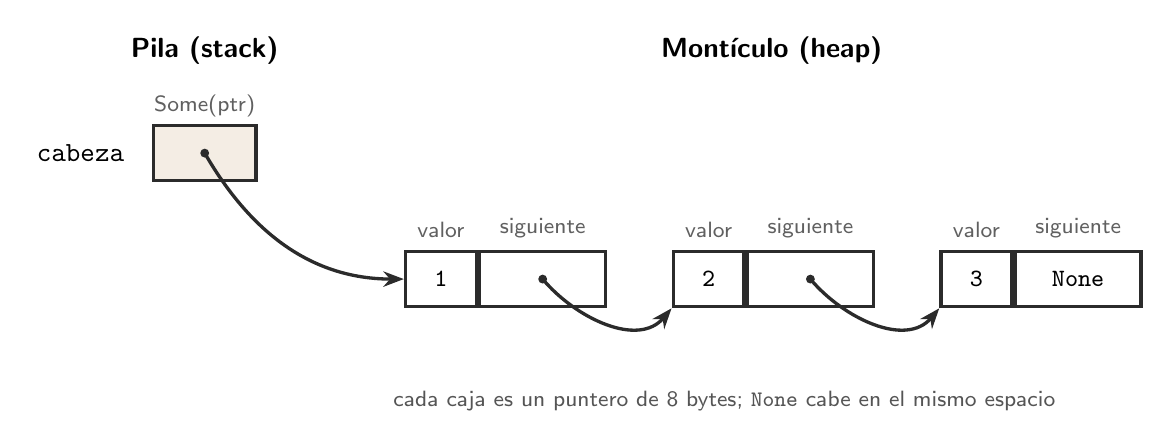
\begin{tikzpicture}[
  celda/.style={draw=carbon,minimum height=7mm,minimum width=13mm,font=\ttfamily\small},
  rotulo/.style={font=\sffamily\footnotesize\color{carbon!75}},
  >={Stealth[length=2.6mm]}]
  % Pila
  \node[font=\sffamily\bfseries] at (0,1.3) {Pila (\textit{stack})};
  \node[celda,fill=arena,very thick] (cab) at (0,0) {};
  \node[rotulo] at (0,0.6) {Some(ptr)};
  \node[anchor=east,font=\ttfamily\bfseries] at (-0.9,0) {cabeza};
  % Montículo: tres nodos
  \node[font=\sffamily\bfseries] at (7.2,1.3) {Montículo (\textit{heap})};
  \foreach \v/\s [count=\i from 0] in {1/{},2/{},3/None} {
    \node[celda,fill=white,very thick,minimum width=9mm] (v\i) at (3.0+\i*3.4,-1.6) {\v};
    \node[celda,fill=white,very thick,minimum width=16mm,anchor=west] (s\i) at (v\i.east) {\s};
    \node[rotulo] at (v\i.north) [above=1pt] {valor};
    \node[rotulo] at (s\i.north) [above=1pt] {siguiente};
  }
  \fill[carbon] (cab.center) circle (1.6pt);
  \draw[->,very thick,carbon] (cab.center) to[out=-60,in=180] (v0.west);
  \fill[carbon] (s0.center) circle (1.6pt);
  \draw[->,very thick,carbon] (s0.center) to[out=-50,in=-130] (v1.south west);
  \fill[carbon] (s1.center) circle (1.6pt);
  \draw[->,very thick,carbon] (s1.center) to[out=-50,in=-130] (v2.south west);
  % Nota
  \node[anchor=north,font=\sffamily\footnotesize,align=center,text=carbon!80] at (6.6,-2.9)
    {cada caja es un puntero de 8 bytes; \texttt{None} cabe en el mismo espacio};
\end{tikzpicture}
\end{document}
